\section{Mini Reed switch (Digital)}
\begin{figure}[H]
    \centering
    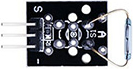
\includegraphics[angle=0, keepaspectratio=true, scale=1, width=200px, height=200px]{images/reed_digital.jpg}
    %\caption{Caption}
\end{figure}
\subsection*{Description}
A reed switch is basically a switch that is activated when a magnetic field is near it. This reed switch is just a simplified version of the above module.
\subsection*{Pin mapping}
This pin mapping corresponds to the pins from left to right with the module pins facing towards you.
\begin{table}[H]
    \centering
    \begin{tabular}{|c|c|c|c|c|}
    \hline
    Index &Label &Type &Name &Description\\ \hline
    0 &S &Digital output &D0 &\\ \hline
    1 & &Source voltage &$V+$ &Module source voltage ($5V$)\\ \hline
    2 &- &Ground &GND &\\ \hline
    \end{tabular}
    %\caption{Caption}
    %\label{tab:my_label}
\end{table}
\subsection*{Operation}
The output voltage at the digital output pin (D0) is low when there is an absence of an external magnetic field. When a magnet enters the vicinity of the reed switch the switch is closed and the output of D0 is set to high.
%\subsection*{Code}
%\lstinputlisting[caption=test]{laser.py}